\RequirePackage[hyphens]{url}

\documentclass[final,a4j,12pt]{jreport}

% 新しいfontの定義? なんだろうこれ
\newfont {\boldmathl}{cmmib10 scaled\magstep1}

% 命令の定義{命令の名前}[引数の個数]
% https://qiita.com/zr_tex8r/items/5067307890d36c0e4882

% \bmを文章中でも使えるように?
\newcommand{\bm}[1]{\mbox{\boldmathl #1}}

% smashは高さを潰す?よくわからん
\newcommand{\lw}[1]{\smash{\lower2.0ex\hbox{#1}}}

% マルチカラムを使うときに必要(だと思う)
\usepackage{multicol}

% 数式系を使うときに必要(だと思う)
\usepackage{amsmath,amssymb}

% これを入れておくと画像等の位置指定をするときに強制的にその場所へ置きたい場合[H]を指定できる
\usepackage{here}

% 数式中でベクトルを太字で表現するときに必要
\usepackage{bm}

% 画像の読み込みに必要
\usepackage[dvipdfmx]{graphicx}

% 各種記号
\usepackage{textcomp}

% 部分的に縦書きをするときに必要
\usepackage{plext}

% 番号付き箇条書き(必要なんだっけ?)
\usepackage{enumerate}

% eps形式でもgraphicxを使うのでは?
\usepackage{epsfig}

% コメントアウト環境を使うために必要(必要性が微妙そう?)
\usepackage{comment}

% 長い表を作るときに必要
\usepackage{longtable}

\usepackage{silence}
% Disable all warnings issued by latex starting with "You have..."
\WarningFilter{latex}{You have requested package}

% Japanese Tate Yoko Gosic Minchoの略らしい
% つまり日本語のゴシック、明朝を縦横で使いたいときのパッケージ?
\usepackage{./stylefile/jtygm}

% 参考文献用? コメントアウトしているのはどういうことだろう
% \usepackage{./stylefile/cite}

% 日本語文字と英字が2:1の幅になるverbatimライクな環境 だそうです
% http://konoyonohana.blog.fc2.com/blog-entry-221.html
% \usepackage{./stylefile/jverb}

% hereってえー、これ上のhereと絶対被ってるでしょ
% \usepackage{./stylefile/here}

% 調べても何も出てこない 何?
% ファイルの中身を見たところ卒論用のスタイルファイルだそうです
\usepackage{./stylefile/bpaper}

% epsファイルを使うものらしい graphicxで良くない? コメントアウトされてるしなぁ
% \usepackage{./stylefile/epsbox}

% ページのヘッダーを作るものっぽい
\usepackage{./stylefile/fancyheadings}

% 表の中で斜線を引くためのもの
% \usepackage{./stylefile/slashbox}

% 並べた図に異なる見出しを付ける
% \usepackage{./stylefile/subfigure}

% 参考文献の管理用? よくわからない
\usepackage[backend=bibtex, style=numeric, sorting=none]{biblatex}

% 文字の後にスペースを入れない,という特別扱いをする文字のリストに"'"を追加する
% よくわからないけどbiblatexを使う場合には入れておいた方が良さそう
% https://oku.edu.mie-u.ac.jp/tex/mod/forum/discuss.php?d=2313
\DeclarePrefChars{'-}

% referenceの参照へのパスだろう
% わざわざディレクトリを分ける意味があるのかはわからないが
\addbibresource{./reference/reference.bib}

% 参考文献出力スタイル
% \bibliographystyle{junsrt}

% 置換マクロらしい
% \genfrac{開き括弧}{閉じ括弧}{分数の横棒の太さ}{数式スタイル}{上}{下}
% これ定義する意味あるのか?
\def\frac#1#2{\genfrac{}{}{}{}{\;#1\;}{\;#2\;}}
\def\dfrac#1#2{\genfrac{}{}{}{0}{\;#1\;}{\;#2\;}}
\def\tfrac#1#2{\genfrac{}{}{}{1}{\;#1\;}{\;#2\;}}
\def\sfrac#1#2{\genfrac{}{}{}{2}{\;#1\;}{\;#2\;}}
\def\ssfrac#1#2{\genfrac{}{}{}{3}{\;#1\;}{\;#2\;}}

% いろいろできる表
\usepackage{tabularx}
% これらは何
\newcolumntype{Y}{>{\centering\arraybackslash}X}
\newcolumntype{Z}{>{\raggedleft\arraybackslash}X}

% URLをそのまま書くとチルダとかが無視されるので\url{http://~~}などと書く
\usepackage{url}
% \renewcommand{\url}{\begingroup \def\UrlLeft{}\def\UrlRight{}\urlstyle{rm}\Url}
\PassOptionsToPackage{hyphens}{url}

% 数式とかで使うのか
\def\so{.\raisebox{1ex}{.}.\quad}
% これ三点のこと? それはamsmathがあれば使えそうだけど
\def\because{\raisebox{1ex}{.}.\raisebox{1ex}{.}\quad}

% 超いらなそう……
\def\Omicron{O}
\def\omicron{o}

% 微分記号ですか dy/dxみたいな
\newcommand{\pdif}[2]{\frac{\partial #1}{\partial #2}}

% 見出し番号の深さを6までに指定
\setcounter{secnumdepth}{6}

% プリアンブルの定義・再定義の開始に用いる
% 特に"@"を含むものについて?
\makeatletter

% subsubsubsectionを定義しているのか
\newcommand{\subsubsubsection}{\@startsection{paragraph}{4}{\z@}
  {1.5\Cvs \@plus.5\Cdp \@minus.2\Cdp}
  {.5\Cvs \@plus.3\Cdp}
  {\reset@font\normalsize\sffamily}
}

% argmaxとargminの定義
\newcommand{\argmax}{\mathop{\rm arg~max}\limits}
\newcommand{\argmin}{\mathop{\rm arg~min}\limits}

% 複数行を枠で囲むため
\usepackage{ascmac}

% pandas.DataFrame.to_latexのため
\usepackage{booktabs}

% for 'subtable' environment
\usepackage{subcaption}

% これはエイリアスっぽい
\def\bs#1{\boldsymbol{#1}}
\def\quot#1{``#1''}
\def\ggn{Google {\it N}-gram}

% ページ上部のマージン
\addtolength{\topmargin}{-15mm}
% ページ左側のマージン
\addtolength{\oddsidemargin}{-15mm}

% ここから文書
\begin{document}
\begin{titlepage}
\thesis
{関係推論能力を有する\\Neural Turing Machine}
{ .}
{萩原 将文 教授}
% {杉本 麻樹 教授}
{4}
{学籍番号 61913674}
{東明 鴻希}
\end{titlepage}
\pagenumbering{roman}

% 目次
\contents

\pagenumbering{arabic}

\abstract
 Neural Turing Machine(NTM)のような外部メモリを持つニューラルネットワークモデルは情報を長期的に保存し活用する能力を持つ一方で、
メモリ内容間の複雑な推論を行う能力に課題がある。
関係ネットワークはエンティティ間の関係を計算でき、高度な推論能力を必要とするタスクを解決可能である。
本論文ではNTMのメモリ構造を保ったまま、メモリ内容に関係推論を適用することを提案する。
これにより既存の関係推論ネットワークよりも高度な忘却方式、説明可能性および拡張性を持つモデルを実現する。 想定される課題に対処するため、二段階の順序整理モジュールも新しく提案する。
一段階目のグラフアテンション構造は時間的に隣接する項目間の推論を行う。二段階目のモジュールはメモリをソートしたのちに全項目間の関係を計算し、関係情報専用のメモリに保存する。
実験結果は

\chapter{はじめに}
ニューラルネットワークモデルの一つであるRecurrent Neural Networks(RNN)は、時系列データの学習に広く用いられる。
入力の順伝播を繰り返す最もシンプルなRNNでは、長時間の入力にわたって逆伝播を計算する中で勾配の値が極端に小さくあるいは大きくなるという問題が発生する。
Long-Short Term Memory(LSTM)\cite{lstm}はゲーティング機構によりこれらの問題に対処した。
また、メモリセルの存在により長時間にわたり情報を保持する能力が向上した。
しかしメモリセルのサイズや複雑さの制限により、多くの情報を長期保持する能力にはまだ限界がある[要出典]。

メモリネットワークはメモリとして利用可能な行列を有し、各時間ステップでの入力情報をメモリに読み書きする能力を学習する。
典型的なメモリネットワークの構造は図\ref{fig:memory_net}
End-To-End Memory Networks\cite{E2E}は入力の埋め込みを外部メモリとして保持することで、入力中の長い時間を隔てた関係を解釈できる。
しかし入力系列の各項目を全て保存する必要があるため、時間方向へのスケーリング能力に課題がある。

\begin{figure}[t]
	\centering
	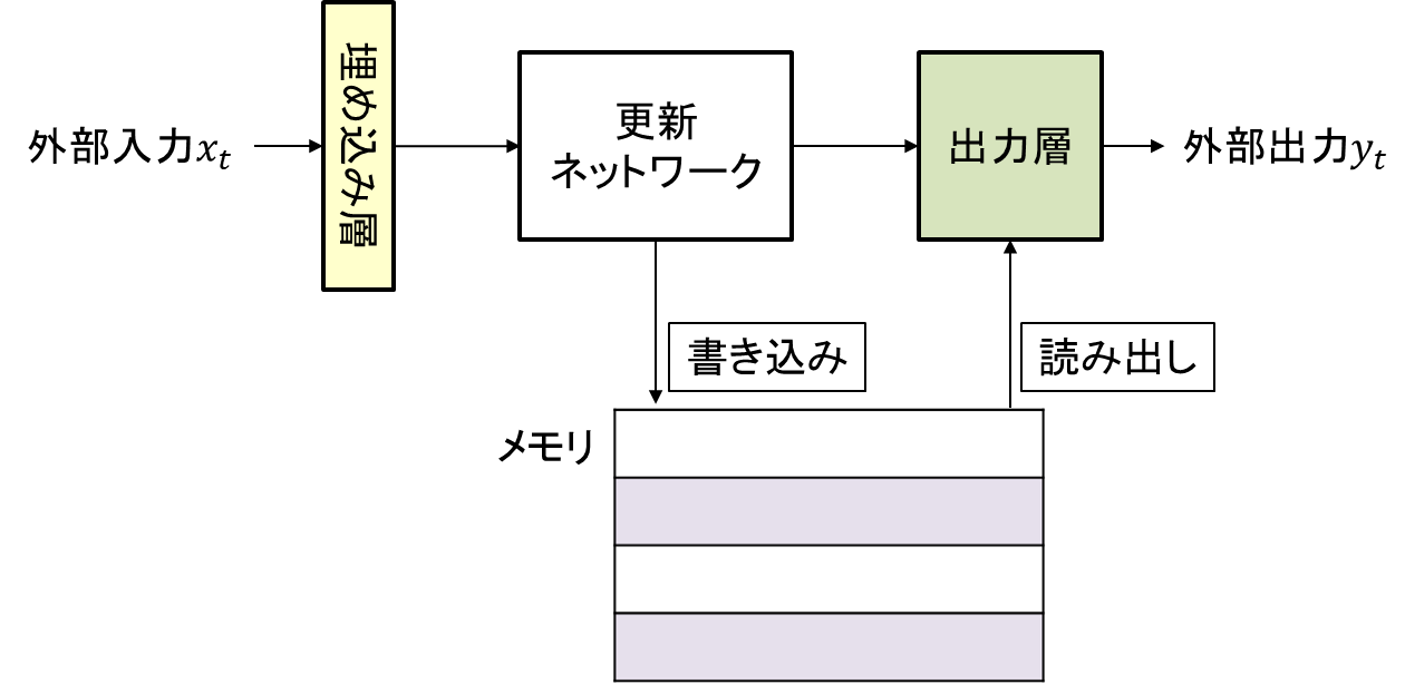
\includegraphics[width=\linewidth]{./figure/img_slide/memory_net.png}
	\caption{典型的なメモリネットワーク}
	\label{fig:memory_net}
\end{figure}

Neural Turing Machine (NTM)\cite{ntm}が有するメモリは固定長であるため、入力の長期化に伴う計算量の増加を回避できる。
メモリスロットの数を超えるサイズの入力系列に対応できるのは、メモリの特定の行を忘却/上書きする能力による。
Differentiable Neural Computer (DNC)\cite{dnc}はNTMの読み出し/書き込み重みの計算部分をより複雑にしたモデルである。
追加モジュールの一つであるusage vectorは、各スロットの使用率を記憶する隠れ状態である。
書き込み重みの算出に利用することで、空いているスロットに優先的に書き込める。
別の追加モジュールであるtemporal link matrixは、スロット間の前後関係を記憶するメモリである。
読み出し重みの計算に利用することで、着目するスロットの前後の時間で書き込まれたスロットも考慮できる。
Convertible Short-Term and Long-Term Memory in DNC (CSLM)\cite{cslm}は、DNCの長期記憶能力をさらに改善する。
メモリの各スロットには重要度が割り振られており、これは学習を通して変化可能である。
重要度の割り当てが低いスロットは忘却されやすく、高いスロットはその逆になる。
これはDNCのメモリがスロット単位で長期記憶と短期記憶に分けられており、その割り当ては適応的かつ学習可能であることを意味する。

これらNTMベースのモデルは学習を通して書き込みの位置や読み出す内容を最適化できる。
しかしメモリの項目間の関係を計算する機構を持たないため、最短経路探索のような入力実体間の関係推論を要求するタスクでの性能に劣る。

関係ネットワークは入力や記憶内の実体間の関係推論能力を持つ。関係の計算はself-attention\cite{transformer}をベースにした手法で行われる。
Relational recurrent neural networks (R-RNN)\cite{rrnn}で提案されたRelational Memory Core(RMC)は、毎時間ステップにおいて入力と全メモリスロット間での関係情報を計算し、その情報でメモリを更新する。
Self-Attentive Associative Memory (SAM)\cite{sam}で提案されたSAM-based Two-memory Model(STM)は、入力を保存する項目メモリと、保存した項目間の関係情報を保存する関係メモリの2種類のメモリを持つ。
項目を忠実に復元することを要求するタスクにおいて、関係メモリのみを持つRMCよりも高い精度を示している。
NTMのように項目がメモリスロット間で区分けされるモデルと異なり、SAMの2つのメモリは分散型のメモリである。
項目メモリは入力のouter productを保存する自己連想記憶、関係メモリは項目メモリから抽出した項目間のouter productを保存する相互連想記憶として実装されており、各入力がメモリ全体に分散するためである。

本論文ではNTMのメモリ構造を保ったまま関係推論モジュールを追加し、メモリ項目間の関係推論能力を追加することを提案する。
関係メモリにはRMCを用いるため、提案ネットワークはNTMを項目メモリ、RMCを関係メモリとして持つ2メモリモデルとなる。
同じ2メモリモデルであるSAMと比較すると、項目メモリが非分散型メモリであり各行で記憶内容が区分けされているある点が異なる。
これにより各入力項目を選択的に忘却・上書きすることが可能になり、R-RNNやSAMのような分散記憶+LSTM方式の忘却よりも高度な忘却が行えると考えられる。
従って長期記憶保持が必要なタスクでより優れた性能を示すことが期待される。
CSLMが各スロットに忘却強度を割り振ったように、読み書き・忘却方式に拡張性・柔軟性があることも利点である。
またこれらのメモリの読み書きはアテンションに由来する説明可能性がある。アテンション係数を可視化することで読み書きした番地を追跡可能である。


この論文の貢献は以下に示す通りである
\\1.NTMに関係推論能力を付与する。このとき関係メモリの入力から一貫性が失われることが予想される。この課題をGATと書き込み頻度ソートの2種類のモジュールにより解決する。
\\2.非分散型のメモリの実装により、分散型メモリよりも長期記憶が必要なタスクに適している。
\\3. 非分散型のメモリにはCSLMに代表されるように拡張性・柔軟性がある。またアテンションを用いる読み書きにより、メモリ操作は説明可能性を持つ。


\chapter{関連研究}

\section{Neural Turing Machine}
NTMの構造は3つのコンポーネントに分けられる。
\\1.情報を保存するメモリ$M_t$は$N×W$次元の行列からなり、これは$W$次元の項目を$N$スロット分保存できる。
\\2.コントローラは毎時間ステップで入力$x_t$を受け取り、隠れ状態$h_t$を計算する。
任意のRNNがコントローラとして採用可能だが、大抵LSTMが用いられる。
\\3.読み出し/書き込みヘッドはコントローラ出力$h_t$とメモリ$M_t$の内容から読み出し/書き込み重みを計算し、メモリへの読み書きを行う。
読み出し/書き込み重みはそれぞれ各スロットへの書き込み/読み出しの強度を表す$N$次元のアテンション係数である。
この重みを計算する操作を”アドレス指定”操作と呼ぶ。

2.1.1節ではヘッドにおける読み書きを説明する。2.1.2節ではアドレス指定を説明する。

\subsection{読み出し/書き込みヘッド}
NTMは読み出し用のヘッドと書き込み用のヘッドそれぞれを1つ以上持ち、ヘッドごとにアドレス指定及び読み書きが行われる。
読み/書き重みをそれぞれ$w^r_t$,$w^w_t$と表し、これらは2.1.2節で説明するアドレス指定操作を用いて計算される。
$w^r_t$,$w^w_t$は式~、~を満たすアテンション係数である。
\begin{equation}
	\sum_{i}w_t(i) = 1
\end{equation}
\begin{equation}
	0\leq w_t(i)\leq 1 , \forall i
\end{equation}
ここで$w_t(i)$は$w_t$のi番目の要素である。メモリからの読み出しは式~のように計算され、読み出しベクトル$r_t$を得る。
\begin{equation}
	r_t = \sum_{i}w_t(i)M_t(i)
\end{equation}
$M_t(i)$は$M_t$のi行目を表す。書き込みは式~による忘却、式~による加算の順で計算され、$M_{t-1}$を$M_t$に更新する。
忘却ベクトル$e_t$、書き込みベクトル$a_t$はコントローラ出力からの変換で得られる。ただし忘却ベクトルの各要素は(0,1)の範囲にある。
\begin{equation}
	M_t'(i) = M_{t-1}(i)[1-w_t(i)e_t]
\end{equation}
\begin{equation}
	M_t(i) = M_t'(i) + w_t(i)a_t
\end{equation}

\subsection{アドレス指定操作}

\section{Relational Memory Core}
関係メモリのベースとして使用した、[R-RNN]で提案されたRMCを説明する。
RMCは毎ステップで入力$x_t$とメモリ$M_{t-1}$の各項目間の関係情報を計算し、そのステップでのメモリ成分$\tilde{M}$を用意する。
LSTMベースのゲーティングを利用して、$\tilde{M}$を$M_{t-1}$に合成し$M_t$を得る。
$\tilde{M}$の計算はマルチヘッドドット積アテンション[Transformer]を用いて行われる。
RMCは項目メモリ$M_i$と入力$x_t$からアテンションを計算するために、クエリ・キー・バリューを計算する為の訓練可能な線形層を有する。
それぞれを$W_q$,$W_k$,$W_v$と表現すると、$\tilde{M}$は式~のようにして計算される。
\begin{equation}
	\tilde{M} =softmax ( \frac{M_{t-1}W_q ([M_{t-1};x_t]W_k)^T}{ \sqrt{d_k}} ) [M_{t-1};x_t]W_v
\end{equation}
ここで$d_k$はキーベクトルの次元 、[M;x]は$M$に$x_t$を新たな行として連結した$(N+1)\times M$次元の行列を表す。クエリ行列の計算では[M:x]ではなく$M$を入力することに注意が必要である。これは$\tilde{M}$の次元を$M_t$と等しくすることを目的としている。

ヘッドが複数存在する時は、ヘッドごとに独立な線形層を用いたアテンション計算結果を結合し最終的な$\tilde{M}$を得る。
各ヘッドの計算結果を$\tilde{M_1},\tilde{M_2}…\tilde{M_h}$と表すとき、それぞれの次元は$N\times (M/h)$であり、$\tilde{M_t}=[\tilde{M_1}: … :\tilde{M_h}]$とすることで$M_t$と同じ次元の$\tilde{M}$を得る。
[:]は行方向の連結を表す。

$\tilde{M}$により$M_t$を更新するためにLSTMを利用する。$M_t$の各行を2D-LSTMの各メモリセルとして実装することで、式x~yによって更新される。$m_i$,$\tilde{m_i}$はそれぞれ$M_t$,$\tilde{M}$の$i$番目の行を表す。
\begin{equation}
	 =
\end{equation}
\begin{equation}
	=
\end{equation}
\begin{equation}
	=
\end{equation}
式~において下線部が示す箇所はLSTMからの変更部分である。関数gは既存研究[R-RNN]に従い、MLP + layer normalizationとして実装した。パラメータ は各$m_i$について共通する。

\chapter{NTMへの関係推論能力の付与}
提案ネットワークは2種類のメモリを持つモデルとして構成される。アーキテクチャの全体図を図\ref{fig:teian_net}に示す。

\begin{figure}[t]
	\centering
	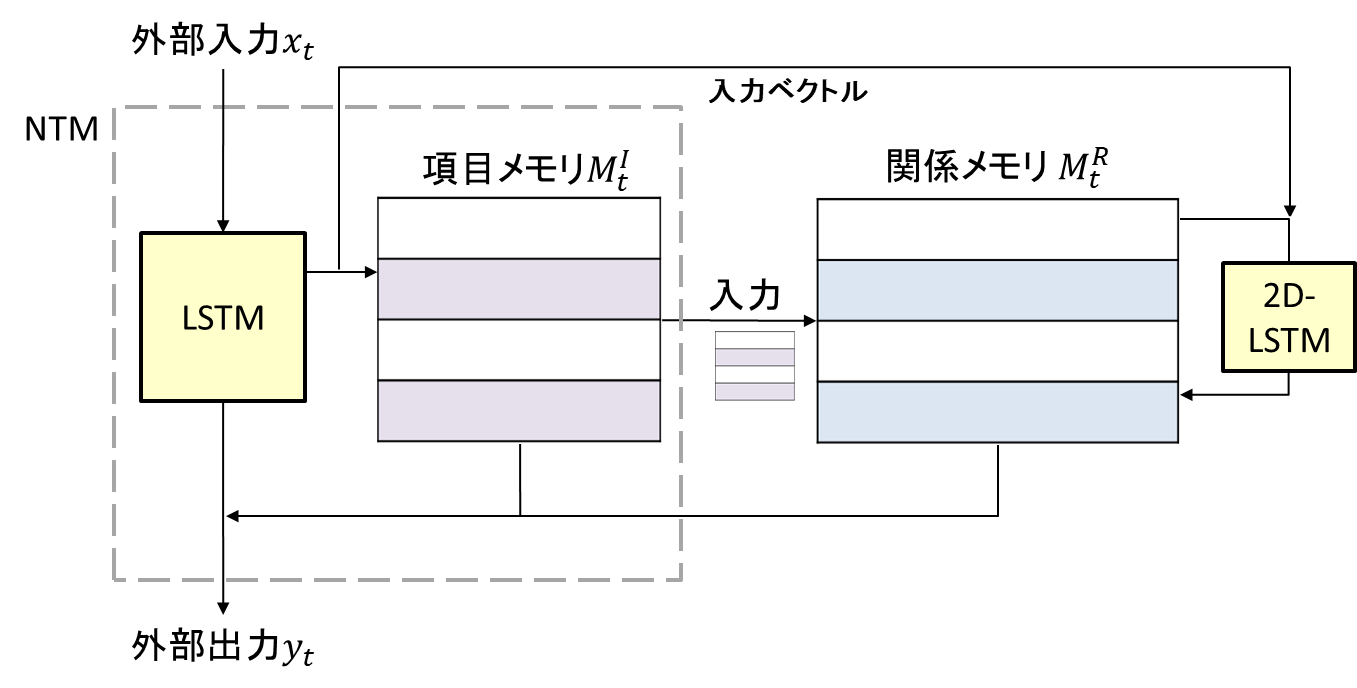
\includegraphics[width=\linewidth]{./figure/img_slide/teian_net.png}
	\caption{提案ネットワーク}
	\label{fig:teian_net}
\end{figure}

ネットワークの構造は大きく3つのモジュールに分けられる。
1つ目は入力の保存・忘却・読み出しを行う項目メモリ$M^I_t$とそのオペレータ。
2つ目は項目メモリの項目間の関係推論を行い、計算した関係情報を保存する関係メモリ$M^R_t$とそのオペレータ。
3つ目は項目メモリの内容を関係メモリに入力する前に項目メモリの項目間順序を整理する順序整理モジュールである。
ネットワークはコントローラLSTMからの出力$o^I_t$、項目メモリからの読み出しベクトル$r^I_t$、関係メモリからの読み出しベクトル$r^R_t$を結合したのちlogistic sigmoid活性化を行い最終的な出力とする。

項目メモリには2.1節で導入したNTMを用いる。関係メモリには2.2節で導入したRMCに変更を加えたものを利用し、この変更は3.1節で説明する。3.2節では新しく提案する順序整理モジュールを2種類説明する。

\section{提案ネットワーク中の関係メモリ}
RMCに変更を加え、項目メモリの各項目間の関係情報を保存する関係メモリとして提案ネットワークに実装する。
提案ネットワーク中の関係メモリは図\ref{fig:teian_rmc}に示すようになる。
時間tにおける関係情報の計算のために、式\ref{eq:rmc_mtil}における入力$x_t$とメモリ$M^R_t$にまたがるアテンションを項目メモリ$M^I_t$と関係メモリ$M^R_t$の連結に対するアテンションに拡張する。
変更後は式\ref{eq:teian_mtil}が示すようにして$\tilde{M}$が計算される。
\begin{equation} \label{eq:teian_mtil}
	\tilde{M} =softmax ( \frac{M_{t-1}W_q ([M_{t-1};M^I_t]W_k)^T}{ \sqrt{d_k}} ) [M_{t-1};M^I_t]W_v
\end{equation}
また$M^R_{t-1}$の更新時には、入力$x_t$の代わりに項目メモリへの書き込みベクトル$w^w_t$を利用する。
従って式\ref{eq:rmc_l2}-\ref{eq:rmc_l4}は式\ref{eq:teian_l2}-\ref{eq:teian_l4}のように変更される。
\begin{equation}\label{eq:teian_l2}
	f_{i,t}=W^f w^w_t +U^f h_{i,t-1}+b^f
\end{equation}
\begin{equation}\label{eq:teian_l3}
	i_{i,t}=W^i w^w_t +U^i h_{i,t-1}+b^i
\end{equation}
\begin{equation}\label{eq:teian_l4}
	o_{i,t}=W^o w^w_t +U^o h_{i,t-1}+b^o 
\end{equation}

\begin{figure}[t]
	\centering
	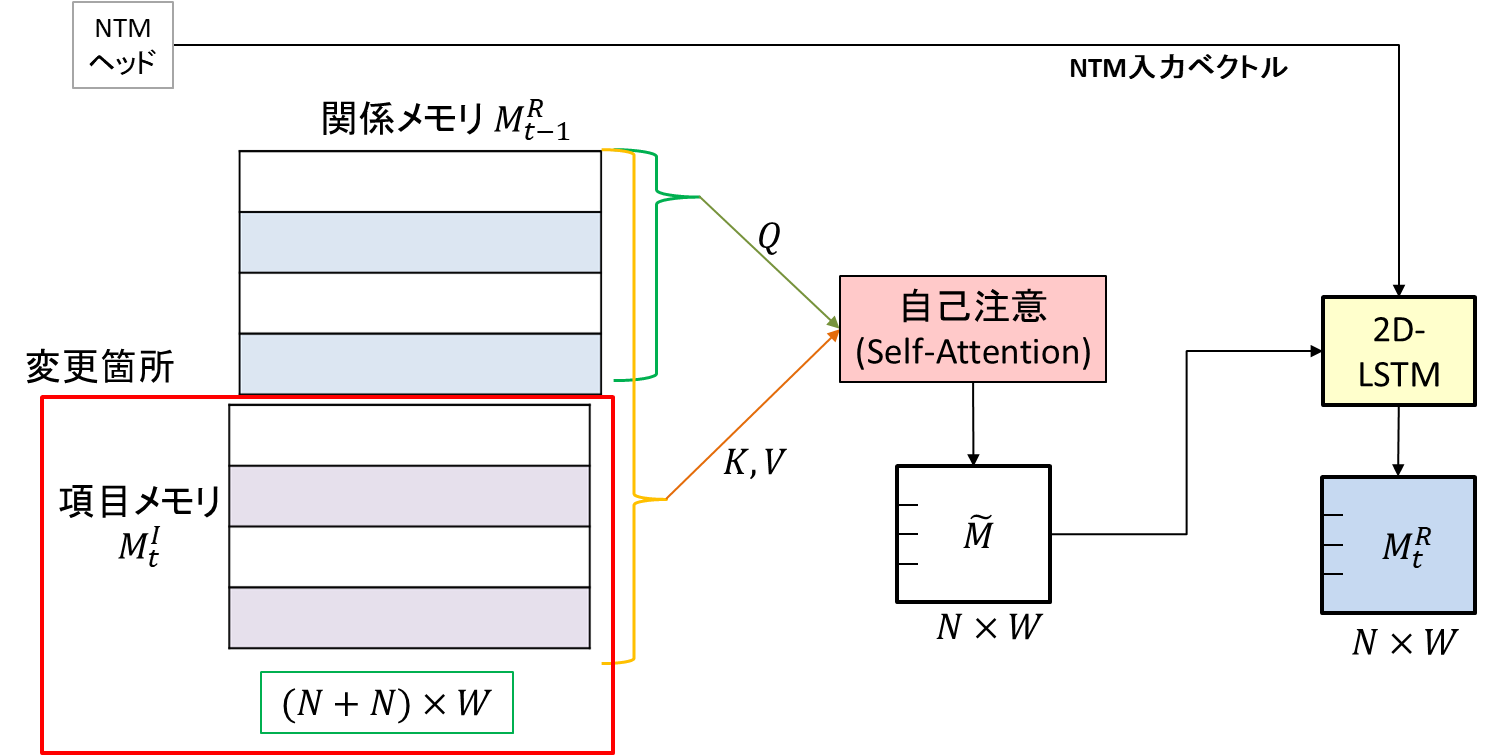
\includegraphics[width=\linewidth]{./figure/img_slide/teian_rmc.png}
	\caption{提案ネットワーク中の関係メモリ}
	\label{fig:teian_rmc}
\end{figure}

\section{順序整理モジュール}
3.2節では項目メモリの順序を解釈・整理する2種類の機構を説明する。3.1節で述べた拡張により、NTMのメモリを関係メモリへの入力とすることが可能となる。
しかしこの実装では項目メモリにおける忘却や上書きは関係メモリの更新と独立して実行されるため、関係メモリへの入力の一貫性が損なわれる問題が予想される。そこで項目メモリを整理し一貫性を持った入力を生成する順序整理モジュールを提案する。

\subsection{書き込み頻度ソート}
項目メモリのヘッドによるメモリの忘却・上書きを疑似的に読み取る手段として、書き込み頻度によるソートを提案する。
時間tにおける各行の書き込み頻度$q_t$($N^I$次元ベクトル)は、式\ref{eq:sum_freq}が示すように$t=1\sim t$での書き込み重みの総和とする。
\begin{equation}\label{eq:sum_freq}
	q_t =\sum_t w^w_t
\end{equation}
関係メモリは式\ref{eq:teian_mtil}において$M^I_t$の代わりに$q_t$に基づいてソートされた$M^I_t$を入力として受け取る。

\subsection{時間リンク行列を利用したグラフアテンション}
DNC\cite{dnc}では各ステップの内容を保存するだけでなく、入力系列内での前後関係の情報を保存するために時間リンク行列を実装している。
時間リンク行列 $L_t$は式\ref{eq:L0}-\ref{eq:L}によって示されるように、時間的に隣接する書き込み重みのouter productionを保存する。
\begin{equation}\label{eq:L0}
	L_0[i,j] =0 \forall i,j
\end{equation}
\begin{equation}\label{eq:Ltii}
	L_t[i,i] =0 \forall i
\end{equation}
\begin{equation}\label{eq:L}
	L_t[i,j] =(1-w^w_t[i]-w^w_t[j])L_{t-1}[i,j]+w^w_t[i]p_{t-1}[j]
\end{equation}
第一項は項目の上書きが発生した時、その位置のリンクをリセットするための項である。
$p_t$は式\ref{eq:prec0},\ref{eq:prec}のようにして計算される。
\begin{equation}\label{eq:prec0}
	p_0 =\boldsymbol{0}
\end{equation}
\begin{equation}\label{eq:prec}
	p_t =(1-\sigma_iw^w_t[i]) p_{t-1}+w^w_t
\end{equation}
提案モジュールでは時間リンク行列を各行が時間的に隣接する程度を表現するグラフと解釈して、グラフアテンション(GAT)\cite{gat}による各項目の変換を試みる。
これにより関係メモリに入力される各項目の特徴量に時間的な順序情報が内包されることが期待できる。
グラフアテンションによる解釈は各行の位置を変更しないため、2.4.1節の書き込み頻度ソートと併用できる。



\chapter{評価実験}\label{chap:evaluation}
全てのタスクにおいてネットワークはLSTMコントローラを採用し、ロジスティックシグモイド出力層を有する。
クロスエントロピーを損失関数として訓練し、最適化手法としてはAdamを用いた。
また、各入力系列の開始時にネットワークの隠れ状態はリセットされる。
各タスクにおけるネットワークのパラメータ、データのバッチサイズ、学習率を付録〜に示す。
実験1・2・4ではビットエラー数が1以下を記録した時点で、実験3では正答率が0.9以上を記録した時点でタスクを解決したとみなし実験を終了した。
\begin{comment}
複数のタスクでネットワークを評価する。実験の目的を以下に示す
\\・4.2節では順序整理モジュールの有効性をablation studyにより検証する
\\・4.3節では提案する非分散型メモリの長期依存関係の計算能力を分散型の既存手法と比較する
\\・4.4節では提案ネットワークにおける関係推論能力を評価する
\\・4.5節ではより複雑な関係推論を必要とするタスクにおける性能をベースラインの関係推論ネットワークと比較する
\end{comment}

\section{実験1 メモリ効率性の検証}
\subsection{実験概要}
NTMとSTMのメモリ操作における,メモリの容量を無駄なく使用する能力(以下メモリ効率性)を比較するためモデルのメモリサイズを揃えて性能を比較した。
評価にはNTM,STMの論文中でも実験で使用されたアルゴリズムタスクであるPriority Sortタスクを用いた。
NTMの論文中ではタスクの入力長が20であるのに対し行数128のメモリを用いて評価を行っている。
本実験ではメモリの容量に余裕のない状態での性能を評価したいため、付録〜に示すようにメモリの行数は入力長と同じ20とした。
比較するSTMのメモリサイズは提案ネットワークと同様に項目メモリ・関係メモリ共に20行とした。
ただしSTMは複数の関係メモリに並列して読み書きを行うことで豊かな関係情報を計算・保存することを長所にしており、
論文中で評価されたモデルでも関係メモリは項目メモリの8倍の大きさを持つ。
そこで関係メモリのサイズを8倍に設定したSTMにおいても実験を行い、性能を比較した。
また、実験1・2では各モデルにおいて2回ずつ独立した学習を行った。

\subsection{タスク:priority sort}
入力系列はランダムなバイナリベクトルに、[-1,1]の範囲から一様分布に従い決定した乱数を優先度として付加したものからなる。
ターゲットは入力系列をこの優先度に従ってソートした系列の一部とする。
NTM中の設定に従い入力系列の長さは20ベクトル,ターゲットは系列の中から優先度が高い順に16ベクトルとする。
評価指標にはビットエラー数を用いた。
これは正規化されたモデルの出力を0.5をしきい値として2値の予測系列に変換した上で、ターゲット系列と異なるビットの数をカウントしたものである。
図\ref{fig:priority}はpriority sortタスクの入力・ターゲットの構成を図示したものである。
\begin{figure}[t]
	\centering
	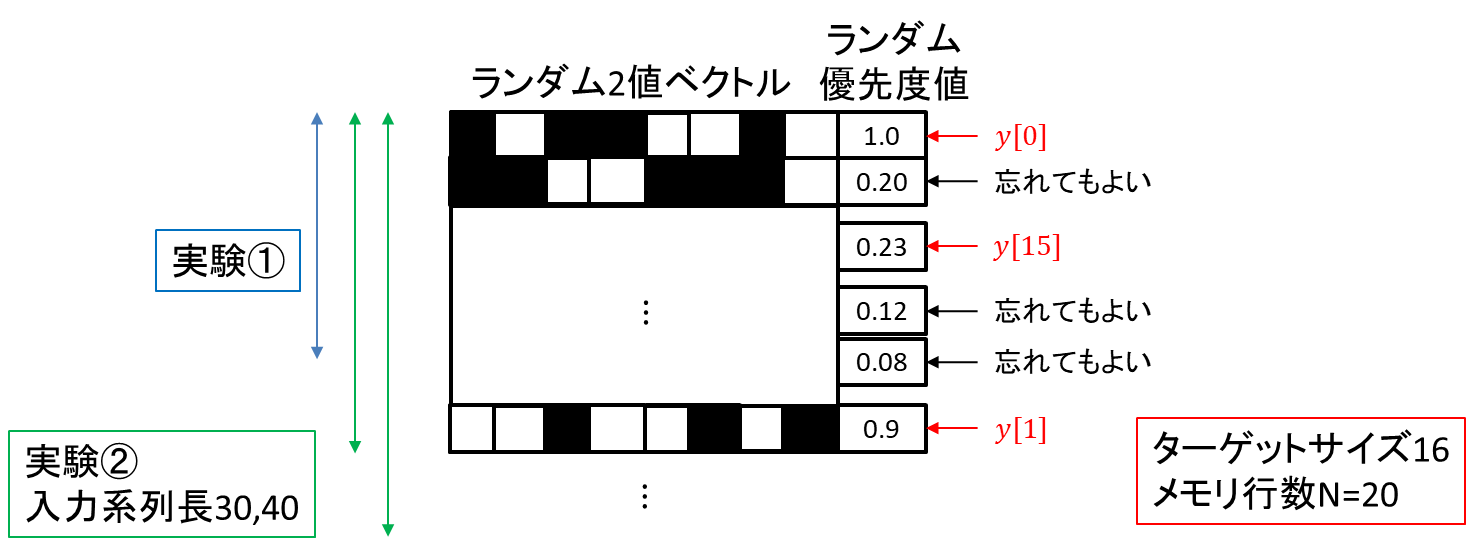
\includegraphics[width=\linewidth]{./figure/img_slide/priority.png}
	\caption{priority sort タスク}
	\label{fig:priority}
\end{figure}

\subsection{実験結果}
Priority SortタスクにおけるNTMおよび提案ネットワークの学習曲線を図\ref{fig:priority_rrnn_m20l20}に示す。
関係メモリが項目メモリと同サイズのSTMの学習曲線を図\ref{fig:priority_samx1_l20}に,
関係メモリサイズが8倍のときのものを図\ref{fig:priority_samx8_l20}に示す。
以後、同色の学習曲線は同一のパラメータ設定下での実験を表す。
\begin{figure}[t]
	\centering
	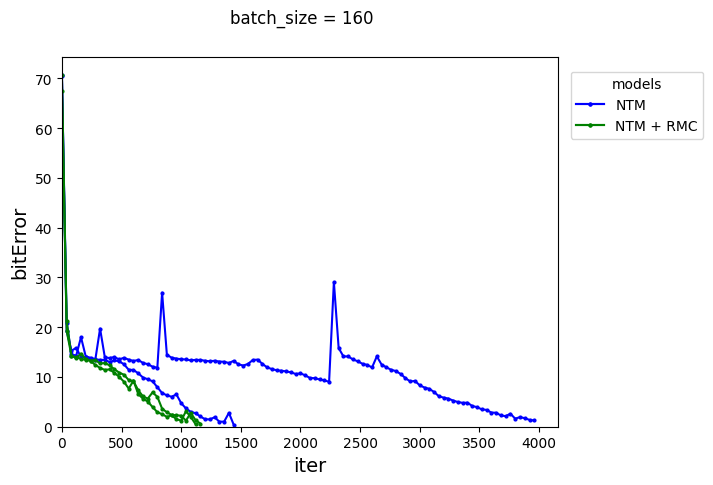
\includegraphics[width=\linewidth]{./figure/priority/rrnn_m20l20.png}
	\caption{NTMおよび提案ネットワークの学習曲線(入力長20)}
	\label{fig:priority_rrnn_m20l20}
\end{figure}
\begin{figure}[t]
	\centering
	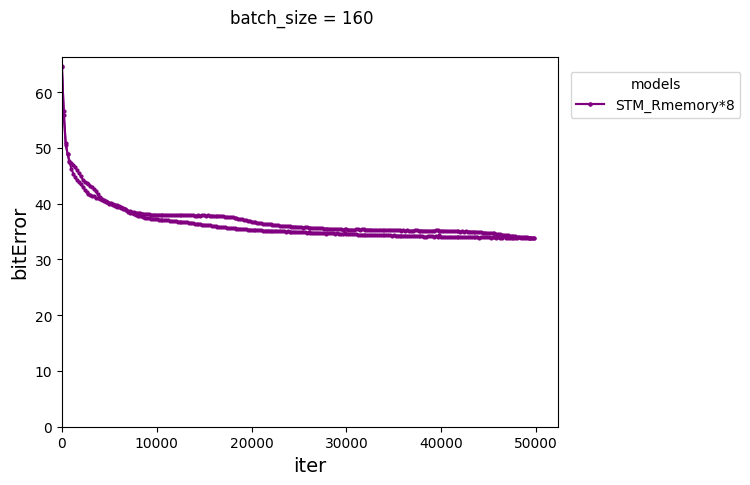
\includegraphics[width=\linewidth]{./figure/priority/samx1l20.png}
	\caption{STMの学習曲線(関係メモリ1倍・入力長20)}
	\label{fig:priority_samx1_l20}
\end{figure}
\begin{figure}[t]
	\centering
	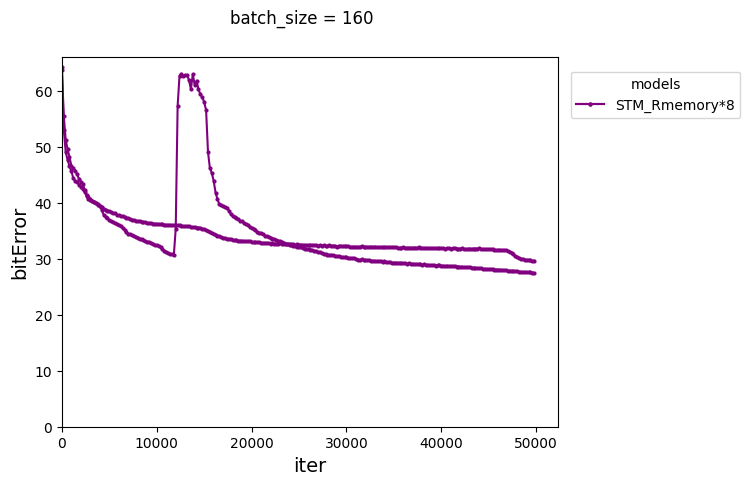
\includegraphics[width=\linewidth]{./figure/priority/samx8l20.png}
	\caption{STMの学習曲線(関係メモリ8倍・入力長20)}
	\label{fig:priority_samx8_l20}
\end{figure}

\subsection{考察}
既存研究よりも大幅にメモリサイズが削減された設定であったが、NTMおよび提案ネットワークはビットエラー数1を下回り、このタスクを解決することが出来た。
STMでは関係メモリのサイズに関わらず、NTM・提案ネットワークの10倍以上のイテレーションで学習した場合でもビットエラー数が30を下回ることは無かった。
これらの結果から、メモリ効率性においてNTMベースのメモリネットワークのSTMに対する優位性が示されたと考えられる。
またNTMは2回の学習のうち1回は学習に不安定性が見られ、収束までに約4000ほどのイテレーションを要した。
一方で提案ネットワークは安定して1200イテレーション未満で収束することに成功しており、これはNTMの最良の結果よりも早期の収束である。

\section{実験2 長期記憶・忘却能力の検証}
\subsection{実験概要}
Priority Sortタスクにおいて入力系列のサイズを増加させたときの精度の推移を観察する。
実験では入力長を30または40に設定した。
ターゲットサイズは16,メモリ行数は20から変更しないため、モデルは依然としてタスクの解決に必要な情報を全て保存する容量を有する。
しかし入力の初期に提示された情報を長期間記憶する能力や優先度の低い不要な項目を選択的に忘却しメモリを再利用する能力が要求される。

\subsection{実験結果}
入力長20,30,40でNTMを訓練したときの学習曲線を図\ref{fig:priority_ntm_m20_l20,30,40}に,
提案ネットワークを訓練したときのものを図\ref{fig:priority_rrnn_m20_l20,30,40}に示す。
同様に関係メモリが項目メモリと同サイズのSTMを訓練したときの学習曲線を図\ref{fig:priority_sam_x1_l20,30,40}に,
関係メモリサイズが8倍のときのものを図\ref{fig:priority_sam_x8_l20,30,40}に示す。
\begin{figure}[t]
	\centering
	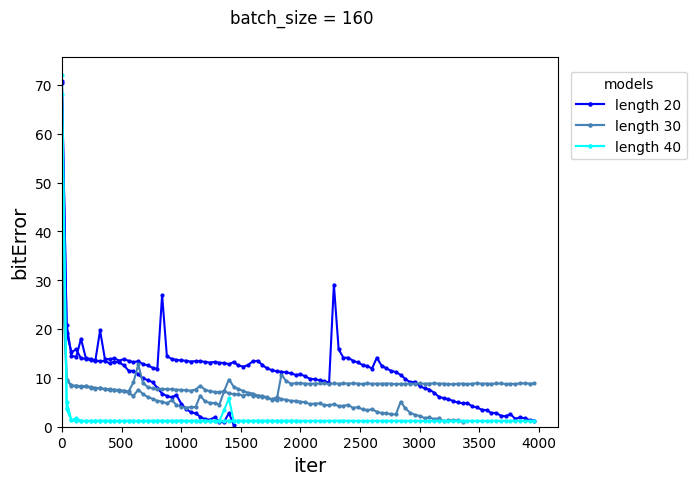
\includegraphics[width=\linewidth]{./figure/priority/ntm_m20_l20,30,40.png}
	\caption{NTMの学習曲線(入力長20,30,40)}
	\label{fig:priority_ntm_m20_l20,30,40}
\end{figure}
\begin{figure}[t]
	\centering
	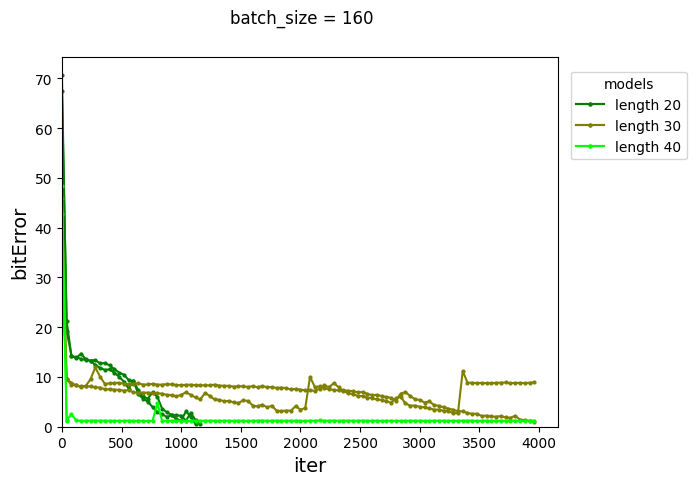
\includegraphics[width=\linewidth]{./figure/priority/rrnn_m20_l20,30,40.png}
	\caption{提案ネットワークの学習曲線(入力長20,30,40)}
	\label{fig:priority_rrnn_m20_l20,30,40}
\end{figure}
\begin{figure}[t]
	\centering
	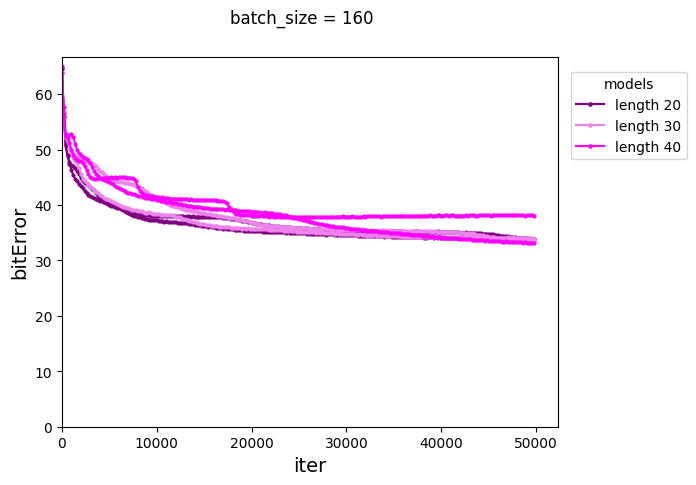
\includegraphics[width=\linewidth]{./figure/priority/sam_x1_l20,30,40.png}
	\caption{STMの学習曲線(関係メモリ1倍・入力長20,30,40)}
	\label{fig:priority_sam_x1_l20,30,40}
\end{figure}
\begin{figure}[t]
	\centering
	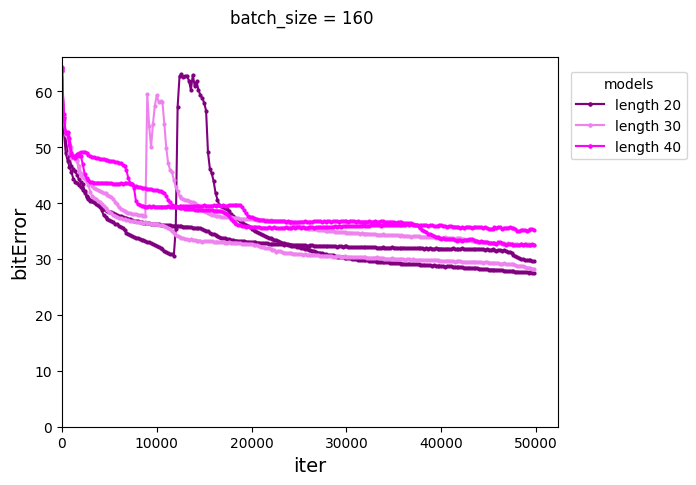
\includegraphics[width=\linewidth]{./figure/priority/sam_x8_l20,30,40.png}
	\caption{STMの学習曲線(関係メモリ8倍・入力長20,30,40)}
	\label{fig:priority_sam_x8_l20,30,40}
\end{figure}

\subsection{考察}
関係メモリが8倍のサイズを持つSTMでは、入力長の増加に伴いエラー率が増加することが読み取れる。
関係メモリが項目メモリと同サイズのSTMでは、イテレーション数が20000以下の範囲ではエラー率に増加が見られるが30000以上では収束し差がなくなる様子が確認できた。
NTMおよび提案ネットワークでは、入力長が30の場合は収束が大幅に遅くなりイテレーション数4000までに解決できない場合も確認された。
ただし、学習初期の500イテレーション以下でのエラー率は入力長20のケースよりも改善されており、最終的なエラー率もSTMの結果に勝っている。
入力長を40とした場合の学習では2回の学習共に非常に早期に収束し、モデルの解決能力は大幅に改善したと言える。

\section{実験3 関係推論能力の評価}
\subsection{実験概要}
この実験の目的は提案手法がNTMに関係推論能力を付与出来るかを評価することである。
実験で用いるNth-farthestタスクにおいて、
既存研究\cite{rrnn}\cite{sam}はRMCやSTMのような関係推論能力を持つモデルが90以上の精度を記録した一方で、NTMやDNCの精度は30を超えないことを示している。
提案ネットワークがNTMメモリ項目間の関係を計算できる場合、NTMよりも大きく改善された精度を示すことが期待される。

\subsection{タスク:Nth-farthest}
入力系列はランダムに生成されたバイナリベクトルからなる。
ベクトルの次元を$d$、系列長を$l$で表したとき、タスクの要求は入力系列中のあるベクトル$m$から$n$番目に遠いベクトルを見つける事である。
$m,n$は入力系列ごとにランダムに決定される。
1ステップあたりの入力はバイナリベクトル、ベクトルのID、$m$、$n$を連結したベクトルからなり、$ID,m,n∈\{1,2,…,l\}$はone-hotエンコーディングにより表現されるため、最終的な入力の次元は$d+3l$になる。
学習に時間を要する実験であったため、入力データの長さ・次元は既存研究\cite{rrnn}の半分の$d=8,l=4$とした。
それに伴い、メモリの大きさも既存研究の半分に設定した。
モデルは正答となるベクトルのIDを出力することを要求されるため、このタスクは分類問題である。評価指標には正答率を用いる。

このタスクは入力の読み書きやソートといったタスクよりも複雑な処理をネットワークに要求する。
ネットワークは$m$と全入力のペアの距離を計算しソートを行う必要がある。距離は入力間の関係情報の一形態である。
入力そのものをソートするタスクと異なり、関係情報のソートの為に関係メモリを活用する必要がある。

\subsection{実験結果}
Nth-farthestタスクによりRMCおよび提案ネットワークを訓練したときの学習曲線を図\ref{fig:nth_result}に示す。
\begin{figure}[t]
	\centering
	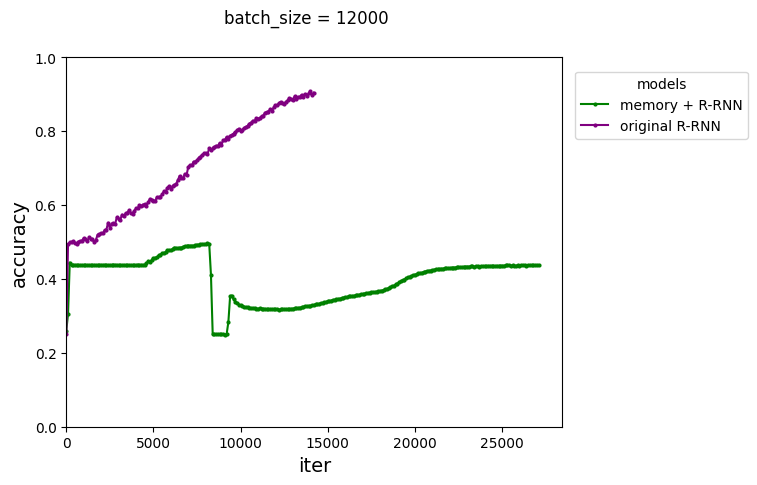
\includegraphics[width=\linewidth]{./figure/nth/orig_rrnn_id1.png}
	\caption{RMCおよび提案ネットワークの学習曲線}
	\label{fig:nth_result}
\end{figure}

\subsection{考察}\label{chap:nth-cons}
実験結果は提案ネットワークの精度は既存手法と異なり90\%に達することはなく、提案ネットワークに関係推論能力は確認されなかった。

原因の一つとして考えられるのは、関係メモリが受け取る情報が不足していたことである。
関係メモリが受け取る入力は項目メモリの保存内容のみであり、
NTMのヘッド内でメモリの更新や読み出しの判断に利用した情報を推論に用いることはない。
改善としてヘッド内で計算した値をメモリ操作を介さず直接関係メモリに渡す経路の追加が考えられる。
特に書き込み重みは、メモリの各行の内容を修飾するのに適した情報であると考えられる。

項目メモリ内の項目の順序に一貫性が無いことが、推論を妨げている可能性も考えられる。
\cite{working2mem}は非分散的に項目を格納する行列に関係推論をかける既存研究の例である。
この論文中のモデルは項目単位の忘却機構を持たず、入力系列に各時間ステップで埋め込みを適用したものを項目記憶として用いる
(論文中では短期記憶として記載されている)。
このため項目は提示された時刻に従って並ぶ一方で、
提案ネットワークでは項目の上書きが発生するため、項目の並び順に一貫性がなくなる可能性がある。
この問題を解決する方法としては、
時間順序に関する情報を別に保存し関係メモリに入力すること、あるいは
時間とは別の基準をもってメモリを一貫性を持った並びに変えることが有効であると考えられる。

また[NTM-implement]はNTMはハイパーパラメータが共通でも、収束までの時間がばらついたり収束に失敗したりする場合があることを指摘している。
提案ネットワークがこうしたNTMの不安定性を引き継ぎ、実験では偶然収束しなかった可能性も考えられる。
同一の設定で何度か追加で学習し、平均精度や収束した回数で評価する必要があると言える。

\section{実験4 関係推論能力改善の検証}
\subsection{実験概要}
\ref{chap:nth-cons}の考察を踏まえ、項目メモリへの書き込みに関する情報を用いて関係メモリの入力を改善し、項目メモリと関係メモリの連携を強化することを試みた。
実験では4種類の異なる方法で変更を加えたモデルの性能をNTMや提案ネットワークと比較し,評価した。
1つ目のモデルでは式\ref{eq:w_sum}で計算される,書き込み重みの総和$q_t$に基づき項目メモリをソートしたものを関係メモリへの入力とした。
このモデルではヘッドにおける計算の内容を直接提示することではなく、関係メモリの入力を一貫性を持った並びにすることを目的としている。
入力系列全体を通して頻繁に提示される項目ほどコンテンツベースの重みによる更新が発生し、$q_t$は大きな値になると考えられる。
そのため関係メモリ内のself-attention入力層の重みは常に同程度の出現頻度の項目を提示されることが期待される。
ヘッドが複数存在する場合、全ヘッドの$q_t$の総和に基づいてソートを行う。
実験4では各モデルにおいて3回ずつ独立した学習を行った。
\begin{equation}\label{eq:w_sum}
	q_t=\sum_t{w^w_t}
\end{equation}
2つ目から4つ目のモデルでは書き込みに関する情報を項目メモリに新たな列として追加し,関係メモリへの入力とした。
ヘッドが複数存在する場合、ヘッドごとに異なる列として追加される。
2つ目では書き込み重みの総和$q_t$を追加した。
3つ目では式\ref{eq:w_sum_thr},\ref{eq:thr}に示すように、書き込み重みの各要素にしきい値処理を適用した値の総和$c_t$を追加した。
書き込み重みの総和を用いる試みでは、一つの行に一つの項目が強く書き込まれた場合と、弱い強度で数回書き込まれた場合の区別を付けることが出来ない。
3つ目の試みは0.1以上の強度の書き込みを全て一度の書き込みとみなし、各行の書き込み回数を保存・利用することを意図したものである。
\begin{equation}\label{eq:w_sum_thr}
	c_t=\sum_tf(w^w_t)
\end{equation}
\begin{equation}\label{eq:thr}
	f(w^w_t)(i)=
	\begin{cases}
	1 & (w^w_t(i) \geq 0.1)\\
	0 & (w^w_t(i) < 0.1)
	\end{cases}
\end{equation}
4つ目では最後に書き込みが行われた時間ステップの情報を項目メモリに追加した。
入力項目が提示された順序の情報を保持し、推論に利用することを目的としている。
付与される時刻は0-1に正規化され、書き込みが行われたかどうかの判定は3つ目の試みと同じく0.1をしきい値とした。

%4.1.1節及び4.1.2節ではネットワークの基礎的な記憶と項目整理の能力を評価する。
%NTM\cite{ntm}の評価で用いられたシンプルなアルゴリズムタスクを説明する。

\subsection{タスク:associative recall}
NTM\cite{ntm}の評価で用いられたシンプルなアルゴリズムタスクの一つである。
一定の長さのランダムに生成されたバイナリベクトルからなる系列を1アイテムとし、
始めにネットワークにはランダムな数のアイテムが入力される。
入力アイテム系列が提示された後、クエリとして入力アイテムのうちの一つが改めて入力される。
この時ターゲットとして、入力アイテムの中でクエリアイテムの次に提示されたアイテムを取る。
各アイテムの間および入力とクエリの間にはデリミタを表すベクトルが挿入される。
NTM\cite{ntm}中の設定に従い、ベクトルの次元を6,1アイテムの長さを3とし、アイテムの数は一様分布を用いて2-6のいずれかに決定する。
評価指標にはPriority Sortと同様にビットエラー数を用いる。

%以上の設定から入力系列の長さはデリミタを含め7-23,デリミタを除いた保存が必要な必要なベクトルに限ると6-18となる。既存研究\cite{ntm}ではメモリ行数は128に設定されており,これは全ての入力を順に保存するのに十分な。同じメモリ行に本実験では行数を12に設定した。

タスクはクエリアイテムをメモリから検索する、入力ベクトルを忠実に復元するといったメモリネットワークの基礎的な能力を要求する。
加えて、入力アイテムの順序の情報を保存する能力も要求する。

\subsection{実験結果}
Associative RecallタスクによりNTMおよび提案ネットワークを訓練した場合の学習曲線を図\ref{fig:ntm,rmc_m12id3}に示す。
\begin{figure}[t]
	\centering
	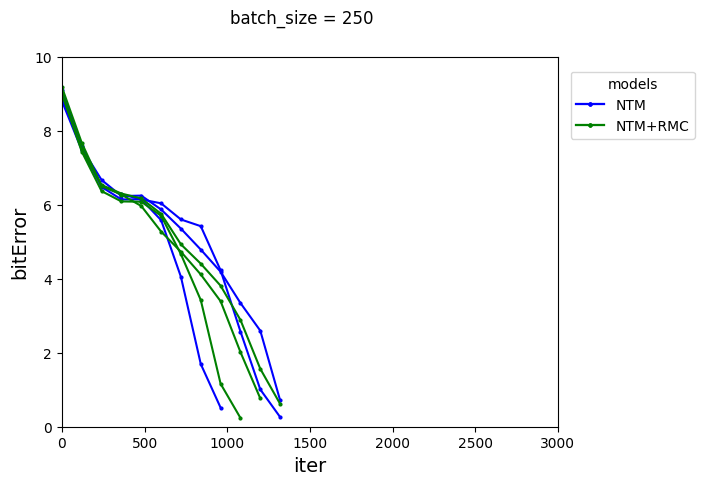
\includegraphics[width=\linewidth]{./figure/associative/ntm,rmc_m12id3.png}
	\caption{NTMおよび提案ネットワークの学習曲線}
	\label{fig:ntm,rmc_m12id3}
\end{figure}

書き込み重みの総和を付与した場合,および総和に従いソートを行った場合の学習曲線をNTMのものと共に図\ref{fig:ntm,sort,supple1}に示す。
各行の書き込み回数,最後に書き込んだ時刻を付与したモデルの学習曲線を図\ref{fig:ntm,supple2,3}に示す。
\begin{figure}[t]
	\centering
	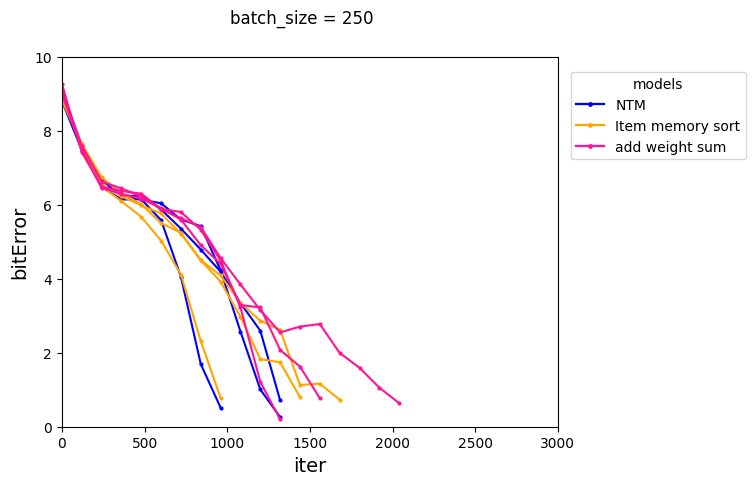
\includegraphics[width=\linewidth]{./figure/associative/ntm,sort,supple1_m12.png}
	\caption{書き込み重みの総和の付与,および総和に従ったソートを行ったときの学習曲線}
	\label{fig:ntm,sort,supple1}
\end{figure}
\begin{figure}[t]
	\centering
	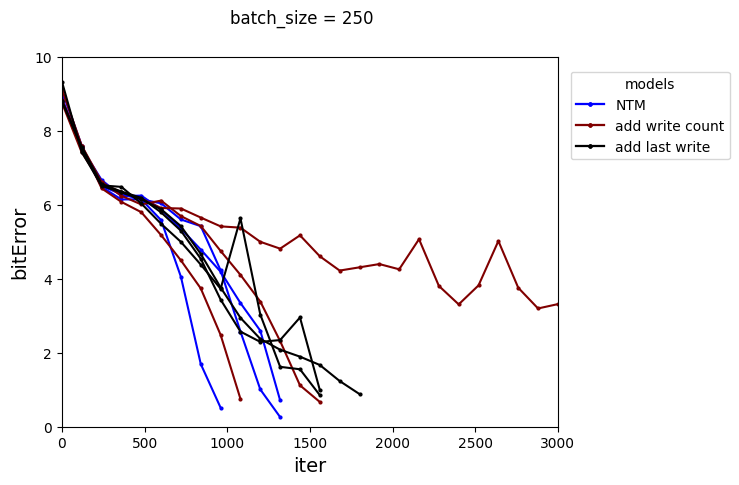
\includegraphics[width=\linewidth]{./figure/associative/ntm,supple2,3_m12.png}
	\caption{各行の書き込み回数,最後に書き込んだ時刻の付与を行ったときの学習曲線}
	\label{fig:ntm,supple2,3}
\end{figure}

\subsection{考察}
結果からこのタスクにおいては、NTMと提案ネットワークの間に顕著な違いは確認されなかった。
重みの総和に基づくソートでも、平均して学習曲線に大きな変化はなかった。
重みの総和あるいは最後に書き込んだ時刻を付与した場合は,平均してエラー率の収束は遅くなったことが読み取れる。
書き込み回数を付与した場合,3回中2回の学習ではNTMに大きくは劣らなかったが1回では収束が大幅に遅れ,モデルの安定性に悪影響を与えたと考えられる。

唯一NTM・提案ネットワークから性能にほぼ悪化が無かったソートを適用したモデルでは、関係メモリの入力の列数に変化はなかった。
性能が悪化した3つのモデルでは関係メモリのサイズに変化はない一方で、各行への書き込みに関する情報として項目メモリに新たな列を付加していた。
これらを比較すると、付加した情報が余分な情報として他の情報が保存されるスペースを圧迫してしまったことが性能悪化の一因と考えられる。
改善として付加される列数=ヘッド数の分関係メモリのサイズを増加させることが考えられる。

最後に書き込んだ時刻および書き込み回数に改善が見られなかった一因として、しきい値処理が逆伝播不可な操作であることも考えられる。
メモリ操作をスキップしてヘッドの情報を関係メモリに渡すことを目的とした操作だが、スキップした接続を通して書き込み重みの計算を最適化可能にする点に改善の余地がある。
しきい値の代わりに急峻なsigmoid関数のような微分可能関数を適用した場合との比較も今後行いたい。

%項目メモリのソートが変化がないのが以外だった。
%self-attentionの変換の重みは位置により機能が分化すると思っていたので。改善か悪化すると思っていた

\begin{comment}
	また,ああああああ


\begin{table}[H]
	\caption{あああといいいの予測誤差}
	\centering
	\scalebox{0.98}[0.98]{
		\begin{tabular}{c|c|c|c|c|c|c}
			\multicolumn{1}{c}{} & \multicolumn{2}{|c|}{2019} 
			& \multicolumn{2}{c|}{2018} & \multicolumn{2}{c}{2017}\\ \hline \hline
			モデル    & ああ & いい & ああ & いい & ああ & いい \\ \hline
			Naive    & \bf{1} & 1 & \bf{1} & 1 & \bf{1} & 1 \\
			TCN      & 1.0895 & 0.9032 & 1.4791 & \bf{0.9198} & 1.2888 & 0.8555 \\
			LSTM     & 1.0384 & 0.9295 & 1.4917 & 0.9725 & 1.1627 & 0.8541 \\
			提案手法  & 1.0977 & \bf{0.8698} & 1.3824 & 0.9439 & 1.2061 & \bf{0.8516} \\
		\end{tabular}
	}
	\label{table:result-1}
\end{table}

\end{comment}
\chapter{結論}
本論文では



記法メモ\\
test\cite{babi} \cite{memory_net} \cite{ntm} \cite{dnc} \cite{cslm} \cite{rrnn} \cite{simple_rel}
\cite{sam} \cite{gat} \cite{working2mem}
Wavenet\cite{oord2016wavenet}は
音声波形を時系列データとして自己回帰モデルで学習することによって,人間の声のような自然な音声を生成することができる.
時点$t$における観測値を$x_t$,$\bm{x} = \left\{ x_1, ..., x_T \right\}$を観測値の全体集合とする.このとき,波形の同時確率は 条件付き確率の積として
以下のよう表現される.
\begin{equation}
	p(\bm{x}) = \prod_{t=1}^T p(x_t | x_1, ..., x_{t-1})
\end{equation}

つまり,$x_t$は前時点の全てにおけるサンプルに条件づけられる.



図\ref{fig:ccl}に因果的畳み込み層のスタックを示す.

\begin{figure}[t]
	\centering
	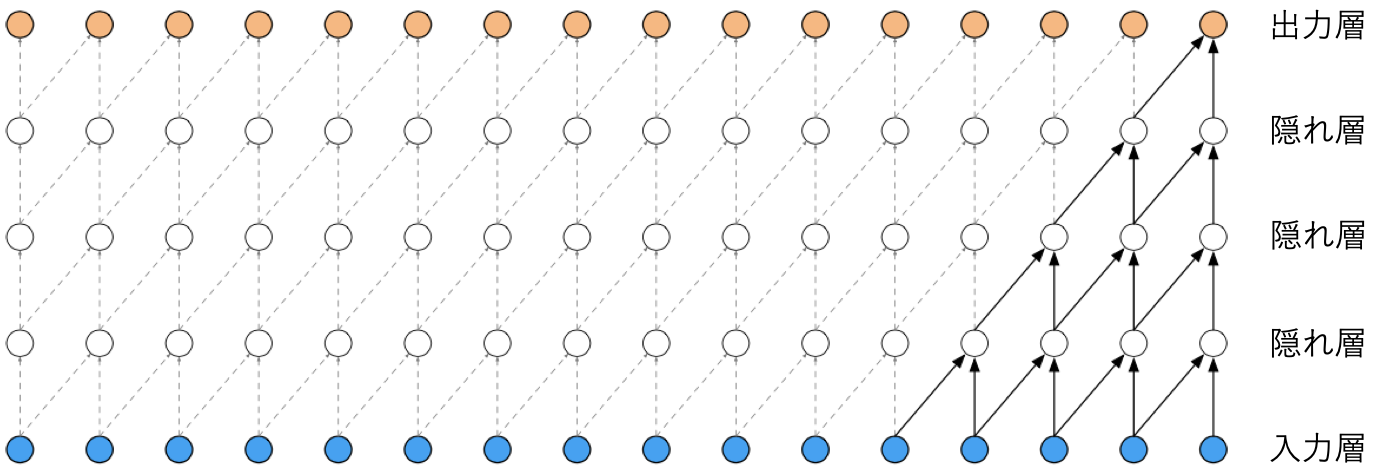
\includegraphics[width=\linewidth]{./figure/ccl.png}
	\caption{因果的畳み込み層}
	\label{fig:ccl}
\end{figure}

\cite{juang1991hidden}は.

今後の課題を以下に挙げる.
\begin{itemize}
	\item の向上
	\par
	必要がある.
	\item への応用
	\par
	を行いたい.
	\newpage
	\item の改善
	\par
	今後,取り組みたい.
\end{itemize}

しかしRMCの追加によって学習にかかる時間が増加し、
学習の高速化

samは項目メモリ内容の間の関係情報を関係メモリに保存する際に、線形変換で圧縮=項目の抽出?をしている。
入力が大きすぎて冗長なのが問題の場合、オートエンコーダのように圧縮・抽出したり、項目メモリ→関係メモリの部分のために読み出し操作をもう一つ実装するとよいかも
でかすぎたか RMCはもともと1ベクトルを入力 無理やり拡張した クエリとの齟齬も

上の実験とは関係なく、実験2の考察を踏まえて、今後修士で試す予定の改善のこともいくつか考えていますがこれらは結論に書く形になると思います。ひとまず以下に箇条書きします
\\関係メモリをRMCではなくSAMにしてみる。もともとRMCは1メモリモデルで入力がベクトルなので、無理に拡張するよりこちらのほうがいいかも
\\SAMや\cite{working2mem}〜のような2メモリモデルを見る限り、関係メモリから項目メモリの内容を復元する操作がある。今は項目→関係の一方向だけど逆も入れてメモリが相互作用できるようにする
\\samは項目メモリ内容の間の関係情報を関係メモリに保存する際に、線形変換で圧縮=項目の抽出?をしている。
入力が大きすぎて冗長なのが問題の場合、オートエンコーダのように圧縮・抽出したり、項目メモリ→関係メモリの部分のために読み出し操作をもう一つ実装するとよいかも
\\似た話としてgraph attentionを利用して時間的・コサイン類似度的に近い項目に重み付けをしたセルフアテンションをかける。この結果を関係メモリに保存する(rmc,SAMとは異なる構造の関係メモリになる)

babi 

また現在の提案ネットワークにおける情報の受け渡しは項目メモリから関係メモリの方向に限定されている。
一方で、既存の2メモリモデルには関係メモリから項目メモリへと情報を渡す経路も存在する。
STMには関係メモリが関連する項目を復元し、項目メモリに改めて書き込む操作が実装されている。
[LTD]は長期記憶と作業記憶からなる2メモリモデルであるが、一方の読み出しベクトルを入力に結合しもう一方の読み書き操作で利用する。
提案ネットワークにもこのような経路を導入し、2つのメモリの連携を強化する改善が考えられる。
Nth-farthestタスクにおいては関係メモリのみを持つRMCにより十分な精度を達成することが示されている。
一方で\cite{sam}では、最短経路や最小全域木の探索タスクや同論文で提案されたRARタスクにおいては2つのメモリの存在が性能を向上させることが示されている。
このようなタスクにおいて、上記の改善が提案ネットワークの性能を改善させる可能性が考えられる。

時間順序に着目すると DNCのlink matrix
\ref{chap:link-matlix}

\chapter*{謝辞}
\addcontentsline{toc}{chapter}{謝辞}
本研究を行うにあたり親身に相談に乗っていただき,ご指導してくださった萩原将文教授,
ならびに共に問題解決,議論,相談に付き合ってくださった研究室の先輩方,同期の皆様に深く感謝いたします.
誠にありがとうございました.

% \addcontentsline{toc}{chapter}{参考文献}
\newpage
\pagestyle{fancyplain}\lfoot{}\cfoot{\thepage}\rhead{}
\lhead{\small \gt 参考文献~~}\chead{} \rhead{}
\addcontentsline{toc}{chapter}{参考文献}
\printbibliography[title=参考文献]

\appendix

% 付録はa, b, c,と見出しを付けていく
\chapter{データの前処理} \label{chap:link-matlix}
提案ネットワークに考えられる課題として、NTM内部で項目の並び順に一貫性が無くなることで、関係メモリの学習を阻害することが予想される。
これは入力との類似度に応じてスロットの忘却・上書きを行う機構や、DNCでは空いた場所から優先的に書き込む機構が関係推論の計算と独立していることによる。
この問題は入力が長期化し、忘却が頻繁に行われる場合により顕著になると考えられる。
メモリ全体を常に一貫性をもって解釈するために、以下の2種類のモジュールを提案する。
全体としてはこれらのモジュールが項目メモリの順序を整理・解釈した後に関係メモリに入力する構造となる。
\\1.DNCの時間リンク行列はスロット間の時間的な前後関係を表すグラフと捉えられる。これを元にメモリ項目にグラフアテンション(GAT)\cite{gat}をかけることで、時間的に局所的な情報(文脈)を考慮した情報へと解釈できる。
\\2.各スロットの書き込み頻度をもとにソートする。
\\End-To-End Memory Networks\cite{E2E}のようにメモリ内でデータが時系列で並ぶモデルやSAM[8]のように項目がメモリ全体に分散するモデルでは学習を通してメモリの解釈は一貫していると考えられるため、順序整理モジュールは新しい取り組みである。{要サーベイ}


\section{ヒストリカルデータ}


\chapter{モデルのパラメータ}

\section{の予測}
表\ref{table:result-1}に
\chapter{のモデル化}

\section{異なる}

あ
\chapter{のヒストグラム}

\section{異なる期間}

図
\end{document}
